% questions.tex —— 2005 年·普通高等学校招生考试·湖南卷·文科 · 题目内容片段（无答案）
% 由 tools/generate_projects.py 依来源总账自 2005/2005_数学真题_湖南文科_试题.md 生成，勿手改（改源 MD 后重跑）

\gkpart{一、选择题：本大题共 10 小题，每小题 5 分，共 50 分．在每小题给出的四个选项中，只有一项是符合题目要求的．}

\begin{question}
\gkti{1}设全集 $U = \{-2, -1, 0, 1, 2\}, A = \{-2, -1, 0\}, B = \{0, 1, 2\}$，则 $(\complement_U A) \cap B =$\mbox{（　　）}

\begin{gkopts}(4)
\task A．$\{0\}$
\task B．$\{-2, -1\}$
\task C．$\{1, 2\}$
\task D．$\{0, 1, 2\}$
\end{gkopts}

\end{question}
\begin{question}
\gkti{2}$\tan 600^\circ$ 的值是\mbox{（　　）}

\begin{gkopts}(2)
\task A．$-\dfrac{\sqrt{3}}{3}$
\task B．$\dfrac{\sqrt{3}}{3}$
\task C．$-\sqrt{3}$
\task D．$\sqrt{3}$
\end{gkopts}

\end{question}
\begin{question}
\gkti{3}函数 $f(x) = \sqrt{1 - 2^x}$ 的定义域是\mbox{（　　）}

\begin{gkopts}(2)
\task A．$(-\infty, 0]$
\task B．$[0, +\infty)$
\task C．$(-\infty, 0)$
\task D．$(-\infty, +\infty)$
\end{gkopts}

\Needspace{0.4\textheight}
\end{question}
\begin{question}
\gkti{4}如图，正方体 $ABCD - A_1B_1C_1D_1$ 的棱长为 1，$E$ 是 $A_1B_1$ 的中点，则 $E$ 到平面 $ABC_1D_1$ 的距离为\mbox{（　　）}
\nopagebreak[4]
\begin{center}% 2005 年湖南卷文科第 4 题配图：正方体 ABCD-A1B1C1D1 与截面辅助线
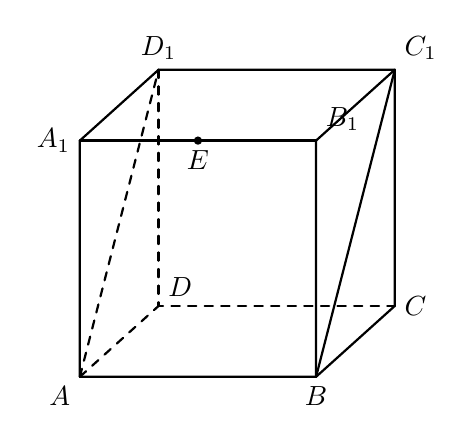
\begin{tikzpicture}[>=latex, line cap=round, line join=round, scale=1.0]
  % 顶点坐标
  \coordinate (A) at (0, 0);
  \coordinate (B) at (3, 0);
  \coordinate (C) at (4, 0.9);
  \coordinate (D) at (1, 0.9);
  
  \coordinate (A1) at (0, 3);
  \coordinate (B1) at (3, 3);
  \coordinate (C1) at (4, 3.9);
  \coordinate (D1) at (1, 3.9);
  
  \coordinate (E) at (1.5, 3);

  % 虚线棱与截面线
  \draw[dashed, thick] (D1) -- (D) -- (C);
  \draw[dashed, thick] (A) -- (D);
  \draw[dashed, thick] (A) -- (D1);

  % 实线棱与截面线
  \draw[thick] (A) -- (B) -- (C) -- (C1) -- (D1) -- (A1) -- cycle;
  \draw[thick] (B) -- (B1) -- (C1);
  \draw[thick] (A1) -- (B1);
  \draw[thick] (B) -- (C1);

  % 点 E
  \fill (E) circle (1.5pt);
  \node[below] at (E) {$E$};

  % 顶点标签
  \node[below left] at (A) {$A$};
  \node[below] at (B) {$B$};
  \node[right] at (C) {$C$};
  \node[above right] at (D) {$D$};
  \node[left] at (A1) {$A_1$};
  \node[above right] at (B1) {$B_1$};
  \node[above right] at (C1) {$C_1$};
  \node[above] at (D1) {$D_1$};
\end{tikzpicture}
\end{center}
\nopagebreak[4]
\begin{gkopts}(2)
\task A．$\dfrac{\sqrt{3}}{2}$
\task B．$\dfrac{\sqrt{2}}{2}$
\task C．$\dfrac{1}{2}$
\task D．$\dfrac{\sqrt{3}}{3}$
\end{gkopts}

\end{question}
\begin{question}
\gkti{5}已知数列 $\{a_n\}$ 满足 $a_1 = 0, a_{n+1} = \dfrac{a_n - \sqrt{3}}{\sqrt{3}a_n + 1}$ ($n \in \mathbf{N}^*$)，则 $a_{20} =$\mbox{（　　）}

\begin{gkopts}(2)
\task A．0
\task B．$-\sqrt{3}$
\task C．$\sqrt{3}$
\task D．$\dfrac{\sqrt{3}}{2}$
\end{gkopts}

\end{question}
\begin{question}
\gkti{6}设集合 $A = \left\{x \ \middle|\ \dfrac{x - 1}{x + 1} < 0\right\}, B = \{x \mid |x - 1| < a\}$，则“$a = 1$”是“$A \cap B \neq \varnothing$”的\mbox{（　　）}

\begin{gkopts}(2)
\task A．充分不必要条件
\task B．必要不充分条件
\task C．充要条件
\task D．既不充分又不必要条件
\end{gkopts}

\end{question}
\begin{question}
\gkti{7}设直线的方程是 $Ax + By = 0$，从 1, 2, 3, 4, 5 这五个数中每次取两个不同的数作为 $A, B$ 的值，则所得不同直线的条数是\mbox{（　　）}

\begin{gkopts}(4)
\task A．20
\task B．19
\task C．18
\task D．16
\end{gkopts}

\end{question}
\begin{question}
\gkti{8}已知双曲线 $\dfrac{x^2}{a^2} - \dfrac{y^2}{b^2} = 1$ ($a > 0, b > 0$) 的右焦点为 $F$，右准线与一条渐近线交于点 $A$，$\triangle OAF$ 的面积为 $\dfrac{a^2}{2}$ ($O$ 为原点)，则两条渐近线的夹角为\mbox{（　　）}

\begin{gkopts}(4)
\task A．$30^\circ$
\task B．$45^\circ$
\task C．$60^\circ$
\task D．$90^\circ$
\end{gkopts}

\end{question}
\begin{question}
\gkti{9}$P$ 是 $\triangle ABC$ 所在平面上一点，若 $\vec{PA} \cdot \vec{PB} = \vec{PB} \cdot \vec{PC} = \vec{PC} \cdot \vec{PA}$，则 $P$ 是 $\triangle ABC$ 的\mbox{（　　）}

\begin{gkopts}(4)
\task A．外心
\task B．内心
\task C．重心
\task D．垂心
\end{gkopts}

\end{question}
\begin{question}
\gkti{10}某公司在甲、乙两地销售一种品牌车，利润（单位：万元）分别为 $L_1 = 5.06x - 0.15x^2$ 和 $L_2 = 2x$，其中 $x$ 为销售量（单位：辆）．若该公司在这两地共销售 15 辆车，则能获得的最大利润为\mbox{（　　）}

\begin{gkopts}(4)
\task A．45.606
\task B．45.6
\task C．45.56
\task D．45.51
\end{gkopts}

\end{question}
\gkpart{二、填空题：本大题共 5 小题，每小题 4 分，共 20 分．把答案填在题中横线上．}

\begin{question}
\gkti{11}设直线 $2x + 3y + 1 = 0$ 和圆 $x^2 + y^2 - 2x - 3 = 0$ 相交于点 $A, B$，则弦 $AB$ 的垂直平分线方程是 $\underline{\qquad\qquad}$．

\end{question}
\begin{question}
\gkti{12}一工厂生产了某种产品 16800 件，它们来自甲、乙、丙 3 条生产线，为检查这批产品的质量，决定采用分层抽样的方法进行抽样，已知甲、乙、丙三条生产线抽取的个体数组成一个等差数列，则乙生产线生产了 $\underline{\qquad\qquad}$ 件产品．

\end{question}
\begin{question}
\gkti{13}在 $(1 + x) + (1 + x)^2 + \dots + (1 + x)^6$ 的展开式中，$x^2$ 项的系数是 $\underline{\qquad\qquad}$．（用数字作答）

\end{question}
\begin{question}
\gkti{14}设函数 $f(x)$ 的图象关于点 $(1, 2)$ 对称，且存在反函数 $f^{-1}(x), f(4) = 0$，则 $f^{-1}(4) = \underline{\qquad\qquad}$．

\end{question}
\begin{question}
\gkti{15}已知平面 $\alpha, \beta$ 和直线 $m$，给出条件：① $m \parallel \alpha$；② $m \perp \alpha$；③ $m \subset \alpha$；④ $\alpha \perp \beta$；⑤ $\alpha \parallel \beta$．

(1) 当满足条件 $\underline{\qquad\qquad}$ 时，有 $m \parallel \beta$；

(2) 当满足条件 $\underline{\qquad\qquad}$ 时，有 $m \perp \beta$．（填所选条件的序号）

\end{question}
\gkpart{三、解答题：本大题共 6 小题，共 80 分．解答应写出文字说明、证明过程或演算步骤．}

\begin{question}
\gkti{16}（本小题满分 12 分）

已知数列 $\{\log_2(a_n - 1)\}$ ($n \in \mathbf{N}^*$) 为等差数列，且 $a_1 = 3, a_3 = 9$．

(1) 求数列 $\{a_n\}$ 的通项公式；

(2) 证明：$\dfrac{1}{a_2 - a_1} + \dfrac{1}{a_3 - a_2} + \dots + \dfrac{1}{a_{n+1} - a_n} < 1$．

\end{question}
\begin{question}
\gkti{17}（本小题满分 12 分）

已知在 $\triangle ABC$ 中，$\sin A(\sin B + \cos B) - \sin C = 0, \sin B + \cos 2C = 0$，求角 $A, B, C$ 的大小．

\Needspace{0.4\textheight}
\end{question}
\begin{question}
\gkti{18}（本小题满分 12 分）

如图 1，已知 $ABCD$ 是上、下底边长分别为 2 和 6，高为 $\sqrt{3}$ 的等腰梯形，将它沿对称轴 $OO_1$ 折成直二面角，如图 2．
\nopagebreak[4]
\begin{center}% 2005 年湖南卷文科第 18 题配图：等腰梯形折成直二面角（图 1 与图 2）
\begin{tikzpicture}[>=latex, line cap=round, line join=round, scale=0.9]
  % ----------------- 图 1 -----------------
  \begin{scope}[shift={(0, 0)}]
    \coordinate (O) at (0, 0);
    \coordinate (A) at (-2.4, 0);
    \coordinate (B) at (2.4, 0);
    \coordinate (O1) at (0, 1.6);
    \coordinate (D) at (-0.8, 1.6);
    \coordinate (C) at (0.8, 1.6);

    \draw[thick] (A) -- (B) -- (C) -- (D) -- cycle;
    \draw[thick] (O) -- (O1);

    \node[below left] at (A) {$A$};
    \node[below right] at (B) {$B$};
    \node[below] at (O) {$O$};
    \node[above] at (O1) {$O_1$};
    \node[above left] at (D) {$D$};
    \node[above right] at (C) {$C$};

    \node[below] at (0, -0.6) {图 1};
  \end{scope}

  % ----------------- 图 2 -----------------
  \begin{scope}[shift={(5.5, 0)}]
    \coordinate (O) at (0, 0);
    \coordinate (O1) at (0, 2.0);
    \coordinate (B) at (2.4, 0);
    \coordinate (C) at (0.8, 2.0);
    \coordinate (A) at (-0.7, -1.0);
    \coordinate (D) at (-0.4, 1.7);

    % 虚线：转折轴 OO1
    \draw[dashed, thick] (O) -- (O1);

    % 实线边与辅助线（AC 与 BO1）
    \draw[thick] (O) -- (B) -- (C) -- (O1);
    \draw[thick] (O) -- (A) -- (D) -- (O1);
    \draw[thick] (B) -- (O1);
    \draw[thick] (A) -- (C);

    % 顶点标签
    \node[below right] at (O) {$O$};
    \node[above] at (O1) {$O_1$};
    \node[right] at (B) {$B$};
    \node[above right] at (C) {$C$};
    \node[below left] at (A) {$A$};
    \node[left] at (D) {$D$};

    \node[below] at (0.8, -1.2) {图 2};
  \end{scope}
\end{tikzpicture}
\end{center}
\nopagebreak[4]
(1) 证明：$AC \perp BO_1$；

(2) 求二面角 $O - AC - O_1$ 的大小．

\end{question}
\begin{question}
\gkti{19}（本小题满分 12 分）

设 $t \neq 0$，点 $P(t, 0)$ 是函数 $f(x) = x^3 + ax$ 与 $g(x) = bx^2 + c$ 的图象的一个公共点，两函数的图象在点 $P$ 处有相同的切线．

(1) 用 $t$ 表示 $a, b, c$；

(2) 若函数 $y = f(x) - g(x)$ 在 $(-1, 3)$ 上单调递减，求 $t$ 的取值范围．

\end{question}
\begin{question}
\gkti{20}（本小题满分 12 分）

某单位组织 4 个部门的职工旅游，规定每个部门只能在韶山、衡山、张家界 3 个景区中任选一个，假设各部门选择每个景区是等可能的．

(1) 求 3 个景区都有部门选择的概率；

(2) 求恰有 2 个景区有部门选择的概率．

\end{question}
\begin{question}
\gkti{21}（本小题满分 14 分）

已知椭圆 $C: \dfrac{x^2}{a^2} + \dfrac{y^2}{b^2} = 1$ ($a > b > 0$) 的左、右焦点为 $F_1, F_2$，离心率为 $e$．直线 $l: y = ex + a$ 与 $x$ 轴、$y$ 轴分别交于点 $A, B$，$M$ 是直线 $l$ 与椭圆 $C$ 的一个公共点，$P$ 是点 $F_1$ 关于直线 $l$ 的对称点，设 $\vec{AM} = \lambda\vec{AB}$．

(1) 证明：$\lambda = 1 - e^2$；

(2) 若 $\lambda = \dfrac{3}{4}$，$\triangle PF_1F_2$ 的周长为 6，写出椭圆 $C$ 的方程；

(3) 确定 $\lambda$ 的值，使得 $\triangle PF_1F_2$ 是等腰三角形．

\end{question}